\documentclass[c]{beamer}
\usepackage[T1]{fontenc}
\usepackage[utf8]{inputenc}
\usepackage{kpfonts}
\usepackage[english]{babel}
\usepackage{animate}
\usepackage{url}
\usepackage{pgfplots}
\usepgfplotslibrary{fillbetween} 
\usepackage{colortbl}
\usepackage{multirow}
\usepackage{hyperref}
\usepackage{bookmark}
\usepackage{dsfont}
\usepackage{csquotes}
\usepackage{amsfonts}
\usepackage{amsmath, amssymb, amsthm}
\usepackage[style=authortitle, maxbibnames=3, minbibnames=3]{biblatex}

\addbibresource{references.bib} 

\usepgfplotslibrary{external}
\tikzexternalize

\pgfmathdeclarefunction{logistic}{1}{%
  \pgfmathparse{1/(1 + exp(-#1))}%
}

\usetheme{Frankfurt}
\useinnertheme{circles}
\useoutertheme[subsection=false]{miniframes}
\usepackage{mycolourtheme}
\usefonttheme{serif}
\addtobeamertemplate{headline}{}{\vskip0.05cm}

\author{Louise Davy}
\institute{Télécom Paris}
\date{\today}
\title{Learning Fair Scoring Functions}
\subtitle{Bipartite Ranking under ROC-based Fairness Constraints}


\AtBeginSection{%
  \begin{frame}
    \frametitle{Outline}
    %\tableofcontents[sectionstyle=show/shaded,hideothersubsections]
    \tableofcontents[sectionstyle=show/shaded,subsectionstyle=hide]
    %\tableofcontents[sectionstyle=show/hide,subsectionstyle=show/shaded/hide]
  \end{frame}
}
\AtBeginSubsection{%
  \begin{frame}<beamer>
    \frametitle{Outline} \tableofcontents[sectionstyle=show/shaded,subsectionstyle=show/shaded/hide]
  \end{frame}
}

\newcommand{\gbf}[1]{\textcolor{secondarycolor}{\textbf{#1}}}

\pgfplotsset{compat=1.18}

\begin{document}
\setbeamertemplate{blocks}[default]
\setbeamertemplate{title page}[default][colsep=-4bp,rounded=false]


\frame[plain]{\titlepage
}

\begin{frame}
  \frametitle{Outline}
  \tableofcontents%[subsectionstyle=hide]
\end{frame}

% INTRODUCTION
\section{Introduction}
\begin{frame}{Introduction}



\begin{block}{\textbf{Paper}}
    \begin{itemize}
        \item \textbf{Title} : Learning Fair Scoring Functions : Bipartite Ranking under ROC-based Fairness Constraints
        \item \textbf{Authors} : Robin Vogel, Aurélien Bellet, Stephan Clémençon
        \item \textbf{Year} : 2021 
        \item \textbf{Arxiv link} : \url{https://arxiv.org/abs/2002.08159}
        \item \textbf{Github link} : \url{https://github.com/RobinVogel/Learning-Fair-Scoring-Functions}
        \item \textbf{Blogpost link} : \url{https://responsible-ai-datascience-ipparis.github.io/posts/lambert-davy/}
    \end{itemize}
\end{block}
    
\end{frame}

% CORPS DE LA PRESENTATION
% Définitions
\section{Definitions}
\subsection{Ranking, bipartite ranking and pairwise bipartite ranking}

\begin{frame}{Ranking}

    {\large\textbf{What is ranking ?}}
    
    Ranking is a class of machine learning algorithms aiming to \gbf{sort} a list of observations according to some \gbf{criterion}. 
    
    \vspace{0.3cm}
    
    {\large\textbf{Examples}}
    
    \begin{itemize}
        \item Information retrieval : Sort documents according to their relevance to a query
        \item Recommendation systems : Recommend user's favourite songs first
    \end{itemize}
\end{frame}

\begin{frame}{Ranking}
    \begin{figure}[H]
        \centering
        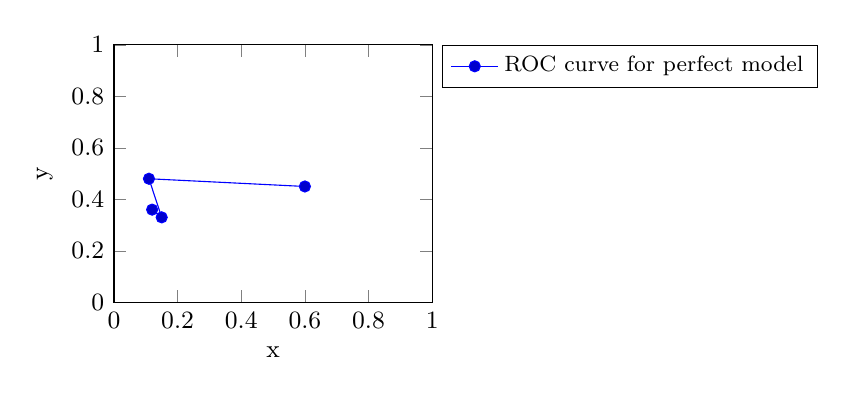
\begin{tikzpicture}
            \begin{axis}[ 
                xlabel=x,
                ylabel=y,
                xmin=0, xmax=1.0,
                ymin=0, ymax=1.0,
                xtick={0,0.2,0.4,0.6,0.8,1.0},
                ytick={0,0.2,0.4,0.6,0.8,1.0},
                legend pos=outer north east,
                height=0.4\textwidth,
                label style={font=\small},
                tick label style={font=\small},
                legend cell align={left},
                legend style={font=\footnotesize,
                            cells={align=left}}
                ] 
                \centering
                \addplot
                coordinates {(0.12,0.36)(0.15,0.33)(0.11,0.48)(0.6,0.45)};
                \addlegendentry{ROC curve for perfect model};
            \end{axis}
        \end{tikzpicture}
    \end{figure}
\end{frame}

\begin{frame}{Bipartite ranking}

    {\large\textbf{What is bipartite ranking ?}}
    
    In bipartite ranking, we consider that all the observations that we want to sort can be partitioned into two classes : \gbf{positive} and \gbf{negative}. We want the positive instances to be consistently \gbf{ranked higher} than the negative ones.
    
    \vspace{0.3cm}

    {\large\textbf{Examples}}
    
    \begin{itemize}
        \item Fraud detection : Find the observations that are most likely to be fraudulent among fraudulent and non-fraudulent observations
        \item Recommendation systems : Recommend user's favourite songs first but this time we have songs that are liked by the user and songs that are disliked
    \end{itemize}
\end{frame}

\begin{frame}{Bipartite ranking}

    {\large\textbf{What is the difference between bipartite ranking and binary classification ?}}

    Bipartite ranking is very close to binary classification since we are trying to distinguish positive instances from negative instances, but \gbf{serves a slightly different goal}. In the cases where a model needs to process a \gbf{large number of observations} and where a \gbf{human verification is needed}, a bipartite ranking model would be able to provide the \gbf{most likely positive instances} first, allowing the human to only investigate a limited number of instances.
    
\end{frame}

\begin{frame}{Bipartite ranking}

    {\large\textbf{What is the difference between bipartite ranking and binary classification ?}}

    There are some works \footcite{narasimhan2013relationship} working around the link between the two that were able to show that a good ranking model, once transferred to binary classification, will perform well (provided that the right threshold was found), while the opposite is not always true. 

    \begin{figure}
        \centering
        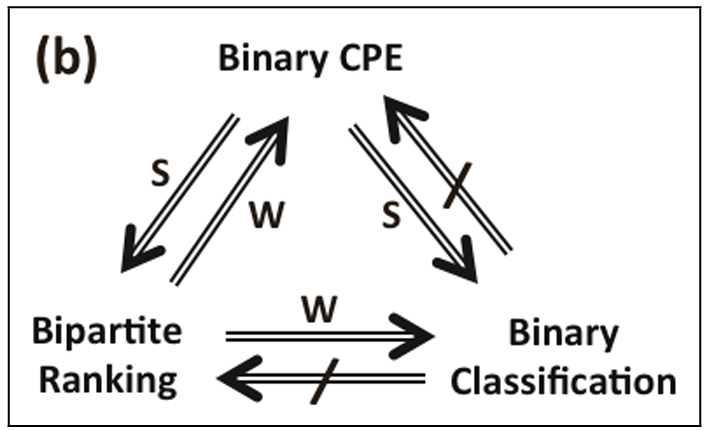
\includegraphics[scale=0.3]{images/link.png}
    \end{figure}
    
\end{frame}

\begin{frame}{Pairwise bipartite ranking}

    {\large\textbf{What is pairwise bipartite ranking ?}}

    Pairwise bipartite ranking is specific case of bipartite ranking, in which we rank each instance \gbf{relatively to another instance}.  Instead of simply distinguishing between positive and negative items, pairwise bipartite ranking considers the \gbf{relative preference between pairs of items}. 

    \vspace{0.3cm}

    {\large\textbf{Example}}
    
    \begin{itemize}
        \item Facial recognition : Find pairs of faces that are the most similar in a database
    \end{itemize}

    \textit{(This is not the focus of this presentation, but this is what I'm currently working on.)}

    
\end{frame}


\subsection{ROC curve and AUC}
\begin{frame}{ROC curve}
    
    {\large\textbf{What is a ROC curve ?}}
    
    ROC stands for \gbf{Receiver Operating Characteristic} curve and is a graph showing the performance of a classification model \gbf{at all classification thresholds}. It plots the false positive rate in the x-axis against the true positive rate in the y-axis. 

    \begin{figure}
        \centering
        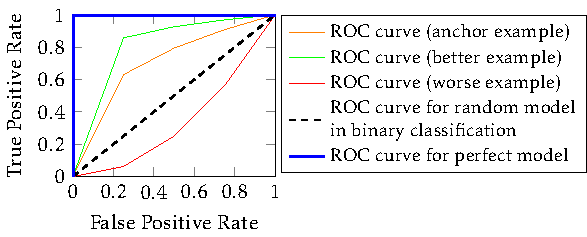
\includegraphics[page=1]{images/output-figure0.pdf}
        \caption{Different ROC curves}
    \end{figure}
    
    % \begin{figure}[H]
    %     \centering
    %     \begin{tikzpicture}
    %         \begin{axis}[ 
    %             xlabel=False Positive Rate,
    %             ylabel=True Positive Rate,
    %             xmin=0, xmax=1.0,
    %             ymin=0, ymax=1.0,
    %             xtick={0,0.2,0.4,0.6,0.8,1.0},
    %             ytick={0,0.2,0.4,0.6,0.8,1.0},
    %             legend pos=outer north east,
    %             height=0.4\textwidth,
    %             label style={font=\small},
    %             tick label style={font=\small},
    %             legend cell align={left},
    %             legend style={font=\footnotesize,
    %                         cells={align=left}}
    %           ] 
    %             \centering 
    %             \addplot[domain=0:1,
    %             samples=5, color = orange]{x^(1/3)};
    %             \addlegendentry{ROC curve (anchor example)};
    %             \addplot[domain=0:1,
    %             samples=5, color = green]{x^(1/9)};
    %             \addlegendentry{ROC curve (better example)};
    %             \addplot[domain=0:1,
    %             samples=5, color = red]{x^2};
    %             \addlegendentry{ROC curve (worse example)};
    %             \addplot[domain=0:1,
    %             samples=10, color = black, thick, dashed]{x};
    %             \addlegendentry{ROC curve for random model \\in binary classification};
    %             \addplot[domain=0:1,
    %             color = blue, {very thick}]
    %             coordinates {(0,0)(0,1)(1,1)};
    %             \addlegendentry{ROC curve for perfect model};
    %       \end{axis}
    %     \end{tikzpicture}
    %     \caption{Different ROC curves}
    % \end{figure}
    
        
\end{frame}


\begin{frame}{AUC}
    
    {\large\textbf{What is the AUC ?}}
    
    AUC stands for \gbf{Area Under the Curve} and is a widely used metric for machine learning model evaluation that quantifies the overall performance of the model \gbf{across all possible classification thresholds}. AUC measures the entire two-dimensional area underneath the entire ROC curve from (0,0) to (1,1). 
    
    {\large\textbf{Example}}
    \begin{itemize}
    	\item A model who is 100\% wrong has an AUC of 0.
    	\item A model who is 100\% correct has an AUC of 1.
    
    \end{itemize}
    
\end{frame}

\begin{frame}{AUC}
    
    {\large\textbf{What is the AUC ?}}

    \begin{figure}
        \centering
        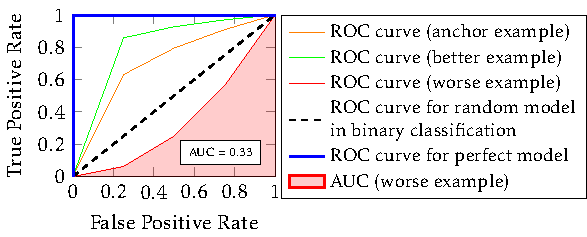
\includegraphics[page=1]{images/output-figure1.pdf}
        \caption{AUC for the worst ROC curve}
    \end{figure}

    
    % \begin{figure}[H]
    %     \centering
    %     \begin{tikzpicture}
    %         \begin{axis}[ 
    %             xlabel=False Positive Rate,
    %             ylabel=True Positive Rate,
    %             xmin=0, xmax=1.0,
    %             ymin=0, ymax=1.0,
    %             xtick={0,0.2,0.4,0.6,0.8,1.0},
    %             ytick={0,0.2,0.4,0.6,0.8,1.0},
    %             legend pos=outer north east,
    %             height=0.4\textwidth,
    %             label style={font=\small},
    %             tick label style={font=\small},
    %             legend cell align={left},
    %             legend style={font=\footnotesize,
    %                         cells={align=left}}
    %           ] 
    %             \centering 
    %             \path[name path=axis] (axis cs:0,0) -- (axis cs:1,0);
    %             \addplot[domain=0:1,
    %             samples=5, color = orange]{x^(1/3)};
    %             \addlegendentry{ROC curve (anchor example)};
    %             \addplot[domain=0:1,
    %             samples=5, color = green]{x^(1/9)};
    %             \addlegendentry{ROC curve (better example)};
    %             \addplot[domain=0:1,
    %             samples=5, color = red, name path=worse_roc]{x^2};
    %             \addlegendentry{ROC curve (worse example)};
    %             \addplot[domain=0:1,
    %             samples=10, color = black, thick, dashed]{x};
    %             \addlegendentry{ROC curve for random model \\in binary classification};
    %             \addplot[domain=0:1,
    %             color = blue, {very thick}]
    %             coordinates {(0,0)(0,1)(1,1)};
    %             \addlegendentry{ROC curve for perfect model};
    %             \addplot [
    %                 thick,
    %                 color=red,
    %                 fill=red, 
    %                 fill opacity=0.2
    %             ]
    %             fill between[
    %                 of=worse_roc and axis,
    %                 soft clip={domain=0:1},
    %             ];
    %             \addlegendentry{AUC (worse example)};
    %             \node[font=\tiny,fill=white,draw,rectangle] at (axis cs: 0.73,0.15) {AUC = 0.33};
    %       \end{axis}
    %     \end{tikzpicture}
    %     \caption{AUC for the worst ROC curve}
    % \end{figure}


\end{frame}

\begin{frame}{AUC}
    
    {\large\textbf{What is the AUC ?}}

    \begin{figure}
        \centering
        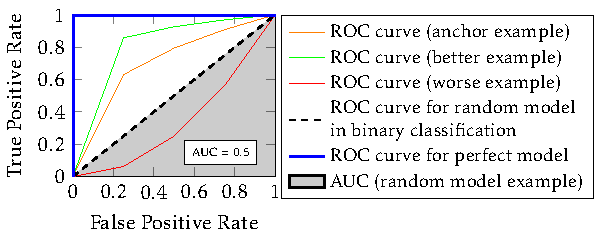
\includegraphics[page=1]{images/output-figure2.pdf}
        \caption{AUC for the random model ROC curve}
    \end{figure}

    % \begin{figure}[H]
    %     \centering
    %     \begin{tikzpicture}
    %         \begin{axis}[ 
    %             xlabel=False Positive Rate,
    %             ylabel=True Positive Rate,
    %             xmin=0, xmax=1.0,
    %             ymin=0, ymax=1.0,
    %             xtick={0,0.2,0.4,0.6,0.8,1.0},
    %             ytick={0,0.2,0.4,0.6,0.8,1.0},
    %             legend pos=outer north east,
    %             height=0.4\textwidth,
    %             label style={font=\small},
    %             tick label style={font=\small},
    %             legend cell align={left},
    %             legend style={font=\footnotesize,
    %                         cells={align=left}}
    %           ] 
    %             \centering 
    %             \path[name path=axis] (axis cs:0,0) -- (axis cs:1,0);
    %             \addplot[domain=0:1,
    %             samples=5, color = orange]{x^(1/3)};
    %             \addlegendentry{ROC curve (anchor example)};
    %             \addplot[domain=0:1,
    %             samples=5, color = green]{x^(1/9)};
    %             \addlegendentry{ROC curve (better example)};
    %             \addplot[domain=0:1,
    %             samples=5, color = red, name path=worst_roc]{x^2};
    %             \addlegendentry{ROC curve (worse example)};
                
    %             \addplot[domain=0:1,
    %             samples=10, color = black, thick, dashed, name path=random_roc]{x};
    %             \addlegendentry{ROC curve for random model \\in binary classification};
    %             \addplot[domain=0:1,
    %             color = blue, {very thick}]
    %             coordinates {(0,0)(0,1)(1,1)};
    %             \addlegendentry{ROC curve for perfect model};
    %             \addplot [
    %                 thick,
    %                 color=black,
    %                 fill=black, 
    %                 fill opacity=0.2
    %             ]
    %             fill between[
    %                 of=random_roc and axis,
    %                 soft clip={domain=0:1},
    %             ];
    %             \addlegendentry{AUC (random model example)};
    %             \node[font=\tiny,fill=white,draw,rectangle] at (axis cs: 0.73,0.15) {AUC = 0.5};
    %       \end{axis}
    %     \end{tikzpicture}
    %     \caption{AUC for the random model ROC curve}
    % \end{figure}


\end{frame}

\begin{frame}{AUC}
    
    {\large\textbf{What is the AUC ?}}

    \begin{figure}
        \centering
        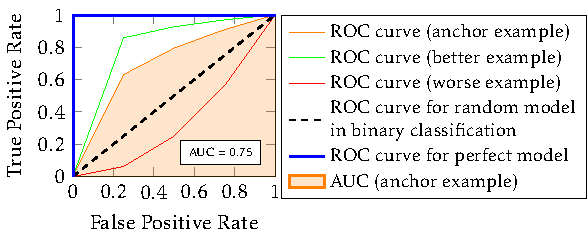
\includegraphics[page=1]{images/output-figure3.pdf}
        \caption{AUC for the anchor ROC curve}
    \end{figure}

    % \begin{figure}[H]
    %     \centering
    %     \begin{tikzpicture}
    %         \begin{axis}[ 
    %             xlabel=False Positive Rate,
    %             ylabel=True Positive Rate,
    %             xmin=0, xmax=1.0,
    %             ymin=0, ymax=1.0,
    %             xtick={0,0.2,0.4,0.6,0.8,1.0},
    %             ytick={0,0.2,0.4,0.6,0.8,1.0},
    %             legend pos=outer north east,
    %             height=0.4\textwidth,
    %             label style={font=\small},
    %             tick label style={font=\small},
    %             legend cell align={left},
    %             legend style={font=\footnotesize,
    %                         cells={align=left}}
    %           ] 
    %             \centering 
    %             \path[name path=axis] (axis cs:0,0) -- (axis cs:1,0);
    %             \addplot[domain=0:1,
    %             samples=5, color = orange, name path = anchor_roc]{x^(1/3)};
    %             \addlegendentry{ROC curve (anchor example)};
    %             \addplot[domain=0:1,
    %             samples=5, color = green, name path = better_roc]{x^(1/9)};
    %             \addlegendentry{ROC curve (better example)};
    %             \addplot[domain=0:1,
    %             samples=5, color = red, name path=worse_roc]{x^2};
    %             \addlegendentry{ROC curve (worse example)};
                
    %             \addplot[domain=0:1,
    %             samples=10, color = black, thick, dashed, name path=random_roc]{x};
    %             \addlegendentry{ROC curve for random model \\in binary classification};
    %             \addplot[domain=0:1,
    %             color = blue, {very thick}]
    %             coordinates {(0,0)(0,1)(1,1)};
    %             \addlegendentry{ROC curve for perfect model};
    %             \addplot [
    %                 thick,
    %                 color=orange,
    %                 fill=orange, 
    %                 fill opacity=0.2
    %             ]
    %             fill between[
    %                 of=anchor_roc and axis,
    %                 soft clip={domain=0:1},
    %             ];
    %             \addlegendentry{AUC (anchor example)};
    %             \node[font=\tiny,fill=white,draw,rectangle] at (axis cs: 0.73,0.15) {AUC = 0.75};
    %       \end{axis}
    %     \end{tikzpicture}
    %     \caption{AUC for the anchor ROC curve}
    % \end{figure}


\end{frame}

\begin{frame}{AUC}
    
    {\large\textbf{What is the AUC ?}}

    \begin{figure}
        \centering
        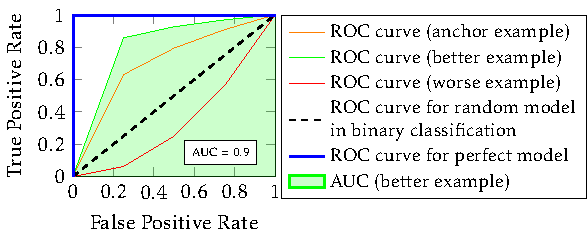
\includegraphics[page=1]{images/output-figure4.pdf}
        \caption{AUC for the better ROC curve}
    \end{figure}

    % \begin{figure}[H]
    %     \centering
    %     \begin{tikzpicture}
    %         \begin{axis}[ 
    %             xlabel=False Positive Rate,
    %             ylabel=True Positive Rate,
    %             xmin=0, xmax=1.0,
    %             ymin=0, ymax=1.0,
    %             xtick={0,0.2,0.4,0.6,0.8,1.0},
    %             ytick={0,0.2,0.4,0.6,0.8,1.0},
    %             legend pos=outer north east,
    %             height=0.4\textwidth,
    %             label style={font=\small},
    %             tick label style={font=\small},
    %             legend cell align={left},
    %             legend style={font=\footnotesize,
    %                         cells={align=left}}
    %           ] 
    %             \centering 
    %             \path[name path=axis] (axis cs:0,0) -- (axis cs:1,0);
    %             \addplot[domain=0:1,
    %             samples=5, color = orange, name path = anchor_roc]{x^(1/3)};
    %             \addlegendentry{ROC curve (anchor example)};
    %             \addplot[domain=0:1,
    %             samples=5, color = green, name path = better_roc]{x^(1/9)};
    %             \addlegendentry{ROC curve (better example)};
    %             \addplot[domain=0:1,
    %             samples=5, color = red, name path=worse_roc]{x^2};
    %             \addlegendentry{ROC curve (worse example)};
                
    %             \addplot[domain=0:1,
    %             samples=10, color = black, thick, dashed, name path=random_roc]{x};
    %             \addlegendentry{ROC curve for random model \\in binary classification};
    %             \addplot[domain=0:1,
    %             color = blue, {very thick}]
    %             coordinates {(0,0)(0,1)(1,1)};
    %             \addlegendentry{ROC curve for perfect model};
    %             \addplot [
    %                 thick,
    %                 color=green,
    %                 fill=green, 
    %                 fill opacity=0.2
    %             ]
    %             fill between[
    %                 of=better_roc and axis,
    %                 soft clip={domain=0:1},
    %             ];
    %             \addlegendentry{AUC (better example)};
    %             \node[font=\tiny,fill=white,draw,rectangle] at (axis cs: 0.73,0.15) {AUC = 0.9};
    %       \end{axis}
    %     \end{tikzpicture}
    %     \caption{AUC for the better ROC curve}
    % \end{figure}


\end{frame}


\begin{frame}{AUC}
    
    {\large\textbf{What is the AUC ?}}

    \begin{figure}
        \centering
        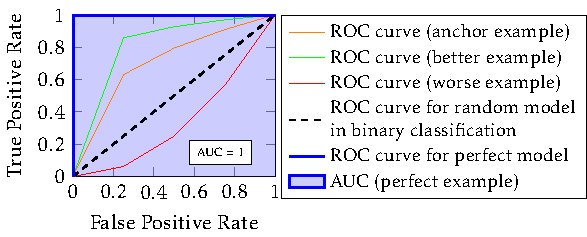
\includegraphics[page=1]{images/output-figure5.pdf}
        \caption{AUC for the perfect ROC curve}
    \end{figure}

    % \begin{figure}[H]
    %     \centering
    %     \begin{tikzpicture}
    %         \begin{axis}[ 
    %             xlabel=False Positive Rate,
    %             ylabel=True Positive Rate,
    %             xmin=0, xmax=1.0,
    %             ymin=0, ymax=1.0,
    %             xtick={0,0.2,0.4,0.6,0.8,1.0},
    %             ytick={0,0.2,0.4,0.6,0.8,1.0},
    %             legend pos=outer north east,
    %             height=0.4\textwidth,
    %             label style={font=\small},
    %             tick label style={font=\small},
    %             legend cell align={left},
    %             legend style={font=\footnotesize,
    %                         cells={align=left}}
    %           ] 
    %             \centering 
    %             \path[name path=axis] (axis cs:0,0) -- (axis cs:1,0);
    %             \addplot[domain=0:1,
    %             samples=5, color = orange, name path = anchor_roc]{x^(1/3)};
    %             \addlegendentry{ROC curve (anchor example)};
    %             \addplot[domain=0:1,
    %             samples=5, color = green, name path = better_roc]{x^(1/9)};
    %             \addlegendentry{ROC curve (better example)};
    %             \addplot[domain=0:1,
    %             samples=5, color = red, name path=worse_roc]{x^2};
    %             \addlegendentry{ROC curve (worse example)};
                
    %             \addplot[domain=0:1,
    %             samples=10, color = black, thick, dashed, name path=random_roc]{x};
    %             \addlegendentry{ROC curve for random model \\in binary classification};
    %             \addplot[domain=0:1,
    %             color = blue, {very thick}, name path = perfect_roc]
    %             coordinates {(0,0)(0,1)(1,1)};
    %             \addlegendentry{ROC curve for perfect model};
    %             \addplot [
    %                 thick,
    %                 color=blue,
    %                 fill=blue, 
    %                 fill opacity=0.2
    %             ]
    %             fill between[
    %                 of=perfect_roc and axis,
    %                 soft clip={domain=0:1},
    %             ];
    %             \addlegendentry{AUC (perfect example)};
    %             \node[font=\tiny,fill=white,draw,rectangle] at (axis cs: 0.73,0.15) {AUC = 1};
    %       \end{axis}
    %     \end{tikzpicture}
    %     \caption{AUC for the perfect ROC curve}
    % \end{figure}


\end{frame}

\subsection{ROC and bipartite ranking}
\begin{frame}{ROC and bipartite ranking}

{\large\textbf{What is the link between ROC curves and bipartite ranking ?}}

\begin{itemize}
    \item Different tasks require different metrics.
    \item \gbf{Classification} : accuracy, precision, recall, f1 score, etc.
    \item \gbf{Regression} : mean squared error, mean absolute error, etc.
    \item \textbf{None of these metrics take the rank into account.} They freeze the number of true/false positives/negatives for a \gbf{particular threshold} (usually 0.5).
    
    \end{itemize} 


\end{frame}


\begin{frame}{ROC and bipartite ranking}


The ROC curve \gbf{intrinsically embeds the information of the rank} by giving information on the confusion matrix for all possible thresholds.

\begin{figure}
    \centering
   
    \animategraphics[autoplay,loop,width=0.5\textwidth]{2}{images/gifs/roc_curve_creation/roc_curve_creation-}{1}{21}
    % ne fonctionne que sur adobe acrobat
    
\end{figure}

Therefore, the analysis of the ROC curve is a \gbf{common solution} to assess the performance of a \gbf{ranking model}.


\end{frame}

        



% Notations

\section{Notations}
\begin{frame}{Notations}

    \begin{itemize}
        \item \textbf{Input space} : $X$, taking values in $\mathcal{X} \subset \mathbb{R}^d$, with $d \geq 1$
        \item \textbf{Output space} : $Y$, taking values in $[-1,+1]$ 
        \item \textbf{Sensitive attribute} : $Z$, taking values in $\{0,1\}$ (when $Z=1$, the individual is part of the sensitive group)
        \item \textbf{Scoring function} : $s : \substack{X \rightarrow Y \\ x \mapsto s(x)}$ 
        \item \textbf{TPR} = True Positive Rate = $\mathbb{P} \{s(X) > t | Y = +1 \}$
        \item \textbf{TNR} = True Negative Rate = $\mathbb{P} \{s(X) \leq t | Y = -1 \}$
        \item \textbf{FPR} =  False Positive Rate = $\mathbb{P} \{s(X) > t | Y = -1 \}$
        \item \textbf{FNR} = False Negative Rate = $\mathbb{P} \{s(X) \leq t | Y = +1 \}$
    \end{itemize}
    
\end{frame}

\begin{frame}{Notations}

    \begin{itemize}
        \item \textbf{Conditional distributions of X given Y} : \\
        $G$ = $\mathbb{P}\{X | Y=+1\}$ \\
        $H$ = $\mathbb{P}\{X | Y=-1\}$
        \item \textbf{Cumulative distribution functions (CDFs)} : \\
        \vspace{-0.85cm} 
        \begin{flalign*}
            G_s(t) &:= \mathbb{P} \{s(X) \leq t | Y = +1 \}&&\\
            &= G(s(X) \leq t)&&\\
            &= \text{\textbf{FNR}}(t) &&
        \end{flalign*} 
        \vspace{-1.1cm}
        \begin{flalign*}
            H_s(t) &:= \mathbb{P} \{s(X) \leq t | Y = -1 \}&&\\
            &= H(s(X) \leq t)&&\\
            &= \text{\textbf{TNR}}(t)&&
        \end{flalign*}   
        
        \vspace{-0.3cm}
        
    \end{itemize}
    
\end{frame}


\begin{frame}{Notations}

    \begin{itemize}
        \item \textbf{ROC curve} : For a fixed \textbf{FPR} that we write  $\alpha \in  [0,1]$ :\\
        \vspace{-0.85cm} 
        \begin{flalign*}
            ROC(\alpha) &:= \text{\textbf{TPR}}(\alpha)&&\\
            &= 1 - \text{\textbf{FNR}} (\text{\textbf{TNR}}^{-1}(1 - \alpha))&&\\ 
            &= 1 - G_s (H_s^{-1} (1- \alpha))&& 
        \end{flalign*}
        \vspace{-0.85cm}
        
        where $\text{\textbf{TNR}}^{-1}(1 - \alpha) = \text{\textbf{FPR}}^{-1}(\alpha) = t_\alpha$.
        \item From now on, we will write $ROC_{H_s,G_s}(\alpha)$.
        \item Why do we use \textbf{FNR} and \textbf{TNR} instead of \textbf{TPR} and \textbf{FPR} ? 
        \item Because they are cumulative distribution functions. 
        \item We can finally define the \textbf{AUC} :\\
        $AUC_{H_s,G_s} = \int_{0}^{1} ROC_{H_s,G_s}(\alpha) d\alpha = \mathbf{P}\{G_s > H_s\} + \frac{1}{2} \mathbf{P}\{G_s = H_s\}$
    \end{itemize}
    
\end{frame}

\begin{frame}{Empirical counterparts}

    \begin{itemize}
        \item \textbf{Training set} : $(X_i,Y_i)_{i=1}^n$ with $n_+$ positive examples and $n_-$ negative examples.
        \item \textbf{Empirical $G_s$ and $H_s$} : \\
        $\widehat{G}_s(t) := (\frac{1}{n_+}) \sum_{i=1}^n \mathds{1}\{ Y_i = +1, s(X_i) \le t \}$\\
        $\widehat{H}_s(t) := (\frac{1}{n_-}) \sum_{i=1}^n \mathds{1}\{ Y_i = -1, s(X_i) \le t\}$
        \item \textbf{Empirical ROC curve} : \\
        $\widehat{ROC}_{H_s, G_s} := ROC_{\widehat{H}_s, \widehat{G}_s} $
        \item \textbf{Empirical AUC} : \\
        \vspace{-0.85cm} 
        \begin{flalign*}
        \widehat{AUC}_{H_s,G_s} 
        &:= AUC_{\widehat{H}_s, \widehat{G}_s}&& \\
        &= \textstyle\frac{1}{n_+ n_-} \sum_{i < j} K( (s(X_i), Y_i), (s(X_j), Y_j))&&
        \end{flalign*} 
        where, for any $t,t' \in \mathbf{R}^2, y,y' \in \{-1,+1\}^2$ :\\
        $K( (t, y), (t', y')) = \mathds{1}\{ (y-y')(t-t') > 0\} + \frac{1}{2}\mathds{1}\{ y \ne y', t=t' \}$ .
    \end{itemize}
    
\end{frame}





% Contributions
\section{Contributions}
\begin{frame}{Contributions}

    The paper addresses the problem of \gbf{fairness} in \gbf{bipartite ranking models}, which have different requirements than classification models.
    
    The authors came up with \gbf{two contributions} to \gbf{improve fairness} of bipartite ranking models :
  \begin{itemize}
      \item AUC-based constraints
      \item ROC-based constraints
  \end{itemize}
  
  They show the \gbf{limitations} of the AUC-based constraints, and how the ROC-based constraints \gbf{address} them.
\end{frame}

\begin{frame}{Motivation}
    Fairness in ranking is important because it can have a significant impact on the decision-making process. For example, in the context of hiring, a biased ranking model can lead to unfair hiring practices.
\end{frame}


\subsection{AUC-based constraints}
\begin{frame}{AUC-based constraints}

\end{frame}

\begin{frame}{Limits of AUC-based constraints}
    \begin{figure}[t]
        \centering
        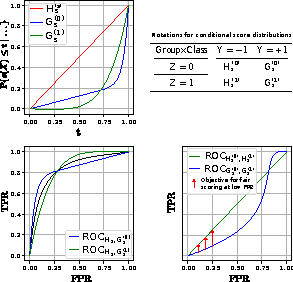
\includegraphics[width=0.6\columnwidth]{images/original_paper/example_simple_dists_explained_with_table2.pdf}
        \caption{Illustrating the limitations of $AUC$-based fairness.}
        \label{fig:example-1}
    \end{figure}
\end{frame}

\subsection{ROC based constraints}
\begin{frame}{ROC based constraints}
    small change
\end{frame}



% Applications
\section{Applications}

\subsection{Compas dataset}
\begin{frame}{Compas dataset}
\end{frame}

\subsection{Adult dataset}
\begin{frame}{Adult dataset}
\end{frame}

% Conclusion
\section{Conclusion}
\begin{frame}{Conclusion}

    ROC based constraints are great
    
\end{frame}

% Bibliography
	\begin{frame}[allowframebreaks]{Bibliography}
		\printbibliography[heading=none].
	\end{frame}

\end{document}